\documentclass[]{book}
\usepackage{lmodern}
\usepackage{amssymb,amsmath}
\usepackage{ifxetex,ifluatex}
\usepackage{fixltx2e} % provides \textsubscript
\ifnum 0\ifxetex 1\fi\ifluatex 1\fi=0 % if pdftex
  \usepackage[T1]{fontenc}
  \usepackage[utf8]{inputenc}
\else % if luatex or xelatex
  \ifxetex
    \usepackage{mathspec}
  \else
    \usepackage{fontspec}
  \fi
  \defaultfontfeatures{Ligatures=TeX,Scale=MatchLowercase}
\fi
% use upquote if available, for straight quotes in verbatim environments
\IfFileExists{upquote.sty}{\usepackage{upquote}}{}
% use microtype if available
\IfFileExists{microtype.sty}{%
\usepackage{microtype}
\UseMicrotypeSet[protrusion]{basicmath} % disable protrusion for tt fonts
}{}
\usepackage[margin=1in]{geometry}
\usepackage{hyperref}
\hypersetup{unicode=true,
            pdftitle={R Lab for Statistical Computing},
            pdfborder={0 0 0},
            breaklinks=true}
\urlstyle{same}  % don't use monospace font for urls
\usepackage{natbib}
\bibliographystyle{apalike}
\usepackage{color}
\usepackage{fancyvrb}
\newcommand{\VerbBar}{|}
\newcommand{\VERB}{\Verb[commandchars=\\\{\}]}
\DefineVerbatimEnvironment{Highlighting}{Verbatim}{commandchars=\\\{\}}
% Add ',fontsize=\small' for more characters per line
\usepackage{framed}
\definecolor{shadecolor}{RGB}{248,248,248}
\newenvironment{Shaded}{\begin{snugshade}}{\end{snugshade}}
\newcommand{\KeywordTok}[1]{\textcolor[rgb]{0.13,0.29,0.53}{\textbf{#1}}}
\newcommand{\DataTypeTok}[1]{\textcolor[rgb]{0.13,0.29,0.53}{#1}}
\newcommand{\DecValTok}[1]{\textcolor[rgb]{0.00,0.00,0.81}{#1}}
\newcommand{\BaseNTok}[1]{\textcolor[rgb]{0.00,0.00,0.81}{#1}}
\newcommand{\FloatTok}[1]{\textcolor[rgb]{0.00,0.00,0.81}{#1}}
\newcommand{\ConstantTok}[1]{\textcolor[rgb]{0.00,0.00,0.00}{#1}}
\newcommand{\CharTok}[1]{\textcolor[rgb]{0.31,0.60,0.02}{#1}}
\newcommand{\SpecialCharTok}[1]{\textcolor[rgb]{0.00,0.00,0.00}{#1}}
\newcommand{\StringTok}[1]{\textcolor[rgb]{0.31,0.60,0.02}{#1}}
\newcommand{\VerbatimStringTok}[1]{\textcolor[rgb]{0.31,0.60,0.02}{#1}}
\newcommand{\SpecialStringTok}[1]{\textcolor[rgb]{0.31,0.60,0.02}{#1}}
\newcommand{\ImportTok}[1]{#1}
\newcommand{\CommentTok}[1]{\textcolor[rgb]{0.56,0.35,0.01}{\textit{#1}}}
\newcommand{\DocumentationTok}[1]{\textcolor[rgb]{0.56,0.35,0.01}{\textbf{\textit{#1}}}}
\newcommand{\AnnotationTok}[1]{\textcolor[rgb]{0.56,0.35,0.01}{\textbf{\textit{#1}}}}
\newcommand{\CommentVarTok}[1]{\textcolor[rgb]{0.56,0.35,0.01}{\textbf{\textit{#1}}}}
\newcommand{\OtherTok}[1]{\textcolor[rgb]{0.56,0.35,0.01}{#1}}
\newcommand{\FunctionTok}[1]{\textcolor[rgb]{0.00,0.00,0.00}{#1}}
\newcommand{\VariableTok}[1]{\textcolor[rgb]{0.00,0.00,0.00}{#1}}
\newcommand{\ControlFlowTok}[1]{\textcolor[rgb]{0.13,0.29,0.53}{\textbf{#1}}}
\newcommand{\OperatorTok}[1]{\textcolor[rgb]{0.81,0.36,0.00}{\textbf{#1}}}
\newcommand{\BuiltInTok}[1]{#1}
\newcommand{\ExtensionTok}[1]{#1}
\newcommand{\PreprocessorTok}[1]{\textcolor[rgb]{0.56,0.35,0.01}{\textit{#1}}}
\newcommand{\AttributeTok}[1]{\textcolor[rgb]{0.77,0.63,0.00}{#1}}
\newcommand{\RegionMarkerTok}[1]{#1}
\newcommand{\InformationTok}[1]{\textcolor[rgb]{0.56,0.35,0.01}{\textbf{\textit{#1}}}}
\newcommand{\WarningTok}[1]{\textcolor[rgb]{0.56,0.35,0.01}{\textbf{\textit{#1}}}}
\newcommand{\AlertTok}[1]{\textcolor[rgb]{0.94,0.16,0.16}{#1}}
\newcommand{\ErrorTok}[1]{\textcolor[rgb]{0.64,0.00,0.00}{\textbf{#1}}}
\newcommand{\NormalTok}[1]{#1}
\usepackage{longtable,booktabs}
\usepackage{graphicx,grffile}
\makeatletter
\def\maxwidth{\ifdim\Gin@nat@width>\linewidth\linewidth\else\Gin@nat@width\fi}
\def\maxheight{\ifdim\Gin@nat@height>\textheight\textheight\else\Gin@nat@height\fi}
\makeatother
% Scale images if necessary, so that they will not overflow the page
% margins by default, and it is still possible to overwrite the defaults
% using explicit options in \includegraphics[width, height, ...]{}
\setkeys{Gin}{width=\maxwidth,height=\maxheight,keepaspectratio}
\IfFileExists{parskip.sty}{%
\usepackage{parskip}
}{% else
\setlength{\parindent}{0pt}
\setlength{\parskip}{6pt plus 2pt minus 1pt}
}
\setlength{\emergencystretch}{3em}  % prevent overfull lines
\providecommand{\tightlist}{%
  \setlength{\itemsep}{0pt}\setlength{\parskip}{0pt}}
\setcounter{secnumdepth}{5}
% Redefines (sub)paragraphs to behave more like sections
\ifx\paragraph\undefined\else
\let\oldparagraph\paragraph
\renewcommand{\paragraph}[1]{\oldparagraph{#1}\mbox{}}
\fi
\ifx\subparagraph\undefined\else
\let\oldsubparagraph\subparagraph
\renewcommand{\subparagraph}[1]{\oldsubparagraph{#1}\mbox{}}
\fi

%%% Use protect on footnotes to avoid problems with footnotes in titles
\let\rmarkdownfootnote\footnote%
\def\footnote{\protect\rmarkdownfootnote}

%%% Change title format to be more compact
\usepackage{titling}

% Create subtitle command for use in maketitle
\providecommand{\subtitle}[1]{
  \posttitle{
    \begin{center}\large#1\end{center}
    }
}

\setlength{\droptitle}{-2em}

  \title{R Lab for Statistical Computing}
    \pretitle{\vspace{\droptitle}\centering\huge}
  \posttitle{\par}
    \author{Young-geun Kim\\
Department of Statistics, SKKU\\
\href{mailto: dudrms33@g.skku.edu}{dudrms33@g.skku.edu}}
    \preauthor{\centering\large\emph}
  \postauthor{\par}
      \predate{\centering\large\emph}
  \postdate{\par}
    \date{2019-03-31}

\usepackage{booktabs}
\usepackage{float}
\usepackage{pdfpages}

\let\oldmaketitle\maketitle
\AtBeginDocument{\let\maketitle\relax}

\usepackage{amsthm}
\newtheorem{theorem}{Theorem}[chapter]
\newtheorem{lemma}{Lemma}[chapter]
\newtheorem{corollary}{Corollary}[chapter]
\newtheorem{proposition}{Proposition}[chapter]
\newtheorem{conjecture}{Conjecture}[chapter]
\theoremstyle{definition}
\newtheorem{definition}{Definition}[chapter]
\theoremstyle{definition}
\newtheorem{example}{Example}[chapter]
\theoremstyle{definition}
\newtheorem{exercise}{Exercise}[chapter]
\theoremstyle{remark}
\newtheorem*{remark}{Remark}
\newtheorem*{solution}{Solution}
\let\BeginKnitrBlock\begin \let\EndKnitrBlock\end
\begin{document}
\maketitle

\begin{titlepage}
  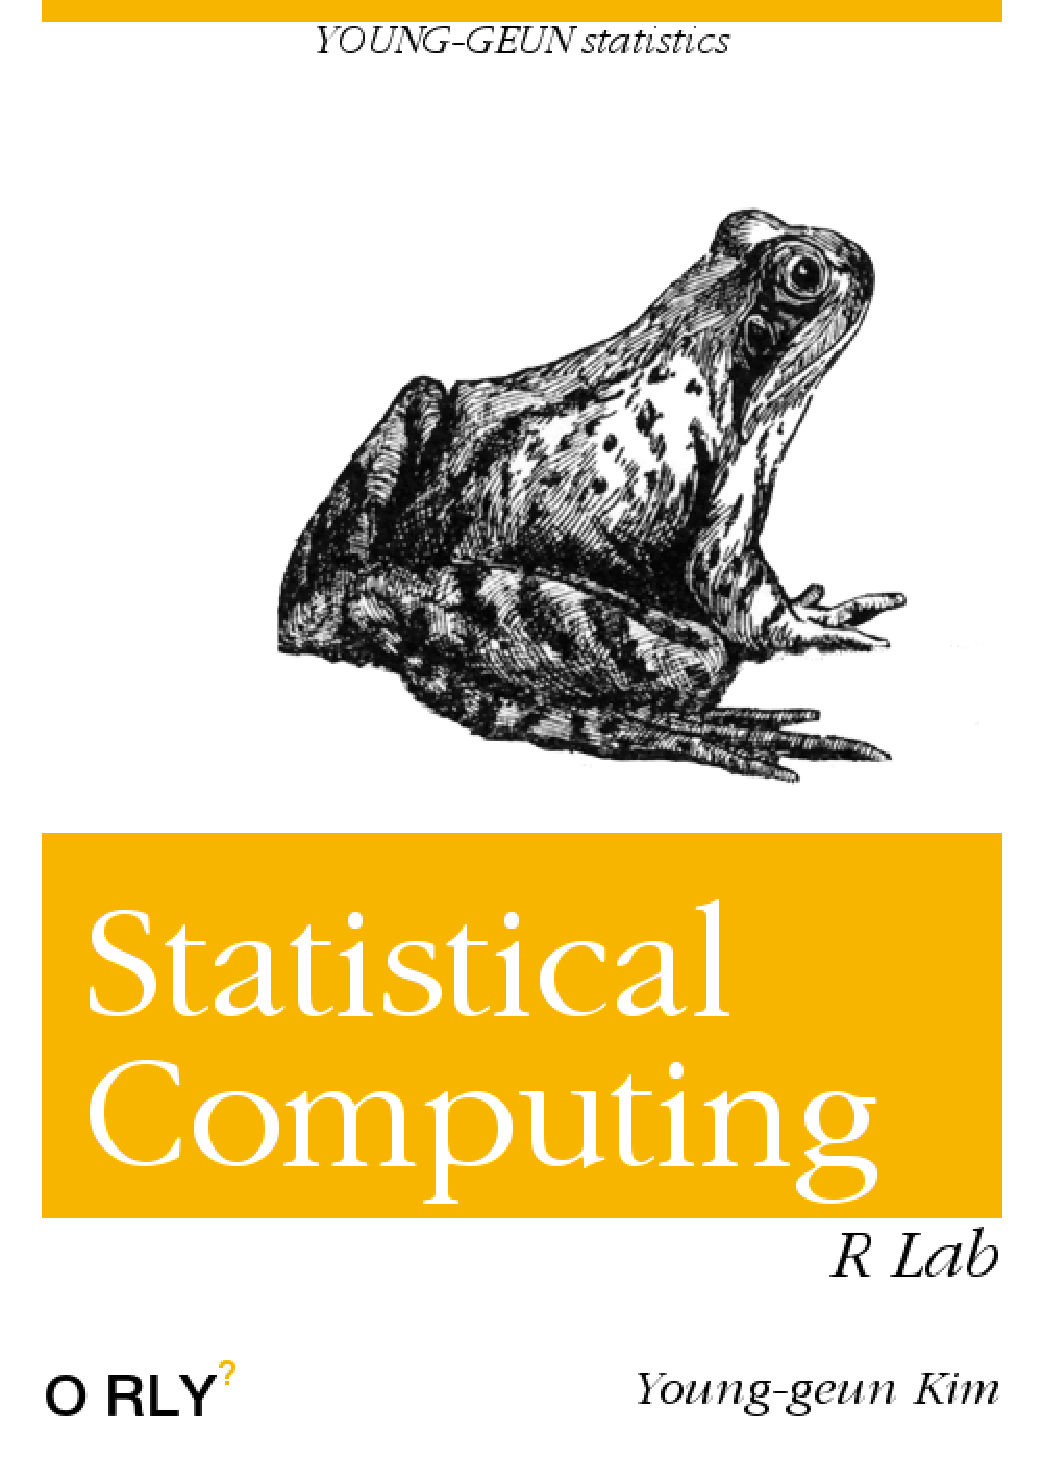
\includepdf{cover.pdf}
\end{titlepage}

\let\maketitle\oldmaketitle
\maketitle

{
\setcounter{tocdepth}{1}
\tableofcontents
}
\chapter*{Statistical Computing}\label{statistical-computing}
\addcontentsline{toc}{chapter}{Statistical Computing}

Statistical computing mainly treats \emph{random generation} methods.
Additionaly, it treats useful simulation methods.

\chapter{Methods for Generating Random Variables}\label{rvar}

\section{Introduction}\label{introduction}

Most of the methods so-called \emph{computational statistics} requires
generation of random variables from specified probability distribution.
In hand, we can spin wheels, roll a dice, or shuffle cards. The results
are chosen randomly. However, we want the same things with computer.
Here, \texttt{r}. As we know, computer cannot generate complete uniform
random numbers. Instead, we generate \textbf{pseudo-random} numbers.

\section{Pseudo-random Numbers}\label{pseudo-random-numbers}

\BeginKnitrBlock{definition}[Pseudo-random numbers]
\protect\hypertarget{def:unnamed-chunk-3}{}{\label{def:unnamed-chunk-3}
\iffalse (Pseudo-random numbers) \fi{} }Sequence of values generated
deterministically which have all the appearances of being independent
\(unif(0, 1)\) random variables, i.e.

\[x_1, x_2, \ldots, x_n \stackrel{iid}{\sim} unif(0, 1)\]
\EndKnitrBlock{definition}

\begin{itemize}
\tightlist
\item
  behave \emph{as if} following \(unif(0, 1)\)
\item
  typically generated from an \emph{initial seed}
\end{itemize}

\subsection{Linear congruential
generator}\label{linear-congruential-generator}

Let \(x_0, x_1, \ldots \in \mathbb{Z}_{+}\).

\begin{enumerate}
\def\labelenumi{\arabic{enumi}.}
\tightlist
\item
  Set \(x_0\) as initial seed.
\item
  Generate \(x_n, n = 1, 2, \ldots\) recursively:

  \begin{enumerate}
  \def\labelenumii{\alph{enumii}.}
  \tightlist
  \item
    \(x_n = (a x_{n - 1} + c) \mod m\)
  \item
    where \(a, c \in \mathbb{Z}_{+}, m: \text{modulus}\)
  \end{enumerate}
\item
  Compute \(u_n = \frac{x_n}{m} \in (0, 1)\)
\end{enumerate}

Then \(u_1, u_2, \ldots \sim unif(0, 1)\)

\begin{Shaded}
\begin{Highlighting}[]
\NormalTok{lcg <-}\StringTok{ }\ControlFlowTok{function}\NormalTok{(n, seed, a, b, m) \{}
\NormalTok{  x <-}\StringTok{ }\KeywordTok{rep}\NormalTok{(seed, n }\OperatorTok{+}\StringTok{ }\DecValTok{1}\NormalTok{)}
  \ControlFlowTok{for}\NormalTok{ (i }\ControlFlowTok{in} \DecValTok{1}\OperatorTok{:}\NormalTok{n) \{}
\NormalTok{    x[i }\OperatorTok{+}\StringTok{ }\DecValTok{1}\NormalTok{] <-}\StringTok{ }\NormalTok{(a }\OperatorTok{*}\StringTok{ }\NormalTok{x[i] }\OperatorTok{+}\StringTok{ }\NormalTok{b) }\OperatorTok\StringTok{ }\NormalTok{m}
\NormalTok{  \}}
\NormalTok{  x[}\OperatorTok{-}\DecValTok{1}\NormalTok{] }\OperatorTok{/}\StringTok{ }\NormalTok{m}
\NormalTok{\}}
\end{Highlighting}
\end{Shaded}

\begin{Shaded}
\begin{Highlighting}[]
\KeywordTok{tibble}\NormalTok{(}
  \DataTypeTok{x =} \KeywordTok{lcg}\NormalTok{(}\DecValTok{1000}\NormalTok{, }\DecValTok{0}\NormalTok{, }\DecValTok{1664525}\NormalTok{, }\DecValTok{1013904223}\NormalTok{, }\DecValTok{2}\OperatorTok{^}\DecValTok{32}\NormalTok{)}
\NormalTok{) }\OperatorTok\StringTok{ }
\StringTok{  }\KeywordTok{ggplot}\NormalTok{(}\KeywordTok{aes}\NormalTok{(}\DataTypeTok{x =}\NormalTok{ x)) }\OperatorTok{+}
\StringTok{  }\KeywordTok{geom_histogram}\NormalTok{(}\KeywordTok{aes}\NormalTok{(}\DataTypeTok{y =}\NormalTok{ ..density..), }\DataTypeTok{bins =} \DecValTok{30}\NormalTok{, }\DataTypeTok{col =} \KeywordTok{gg_hcl}\NormalTok{(}\DecValTok{1}\NormalTok{))}
\end{Highlighting}
\end{Shaded}

\begin{center}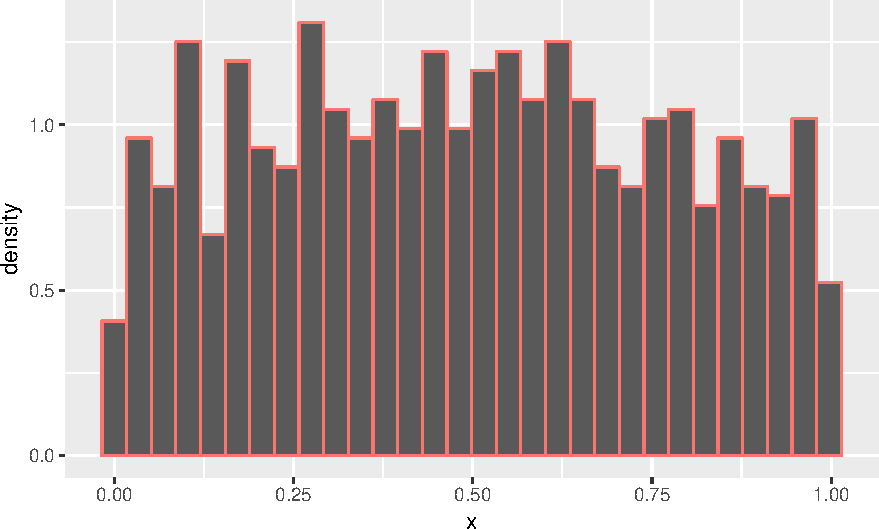
\includegraphics[width=0.7\linewidth]{statistical-computing_files/figure-latex/unnamed-chunk-5-1} \end{center}

\subsection{Multiplicative congruential
generator}\label{multiplicative-congruential-generator}

\subsection{Sampling from a finite
population}\label{sampling-from-a-finite-population}

From finite population, we can sample data with or without replacement.

\begin{Shaded}
\begin{Highlighting}[]
\KeywordTok{sample}\NormalTok{(}\DecValTok{0}\OperatorTok{:}\DecValTok{1}\NormalTok{, }\DataTypeTok{size =} \DecValTok{10}\NormalTok{, }\DataTypeTok{replace =} \OtherTok{TRUE}\NormalTok{)}
\end{Highlighting}
\end{Shaded}

\begin{verbatim}
 [1] 1 0 0 1 0 1 1 0 1 1
\end{verbatim}

\begin{Shaded}
\begin{Highlighting}[]
\KeywordTok{sample}\NormalTok{(}\DecValTok{1}\OperatorTok{:}\DecValTok{100}\NormalTok{, }\DataTypeTok{size =} \DecValTok{6}\NormalTok{, }\DataTypeTok{replace =} \OtherTok{FALSE}\NormalTok{)}
\end{Highlighting}
\end{Shaded}

\begin{verbatim}
[1] 61 83 50 74 34 35
\end{verbatim}

\section{The Inverse Transform
Method}\label{the-inverse-transform-method}

\BeginKnitrBlock{theorem}[Probability Integral Transformation]
\protect\hypertarget{thm:probint}{}{\label{thm:probint}
\iffalse (Probability Integral Transformation) \fi{} }If \(X\) is a
continuous random variable with cdf \(F_(x)\), then
\[U \equiv F_X(X) \sim unif(0, 1)\]
\EndKnitrBlock{theorem}

\BeginKnitrBlock{proof}[Probability Integral Transformation]
\iffalse{} {Proof (Probability Integral Transformation). } \fi{}Let
\(U \sim unif(0, 1)\). Then

\[
\begin{aligned}
P(F_X^{-1}(U) \le x) & = P(\inf\{t : F_X(t) = U \} \le x) \\
& = P(U \le F_X(x)) \\
& = F_U(F_X(x)) \\
& = F_X(x)
\end{aligned}
\]
\EndKnitrBlock{proof}

Thus, to generate \(n\) random variables \(\sim F_X\),

\begin{enumerate}
\def\labelenumi{\arabic{enumi}.}
\tightlist
\item
  form of \(F_X^{-1}(u)\)
\item
  For each \(i = 1, 2, \ldots, n\):

  \begin{enumerate}
  \def\labelenumii{\alph{enumii}.}
  \tightlist
  \item
    Generate \(u_i \sim unif(0, 1)\)
  \item
    \(x_i = F_X^{-1}(u_i)\)
  \end{enumerate}
\end{enumerate}

Collect \(x_1, x_2, \ldots, x_n \sim F_X\).

\subsection{Continuous case}\label{continuous-case}

Denote that the \emph{probability integral transformation} holds for a
continuous variable. When generating continuous random variable,
applying above algorithm might work.

\BeginKnitrBlock{example}[Exponential distribution]
\protect\hypertarget{exm:expon}{}{\label{exm:expon} \iffalse (Exponential
distribution) \fi{} }If \(X \sim Exp(\lambda)\), then
\(F_X(x) = 1 - e^{-\lambda x}\). We can derive the inverse function of
cdf \[F_X^{-1}(u) = \frac{1}{\lambda}\ln(1 - u)\]
\EndKnitrBlock{example}

From above example \ref{exm:expon}, we just type the inverse cdf in the
function to use the method.

\begin{Shaded}
\begin{Highlighting}[]
\NormalTok{inv_exp <-}\StringTok{ }\ControlFlowTok{function}\NormalTok{(n, lambda) \{}
  \OperatorTok{-}\KeywordTok{log}\NormalTok{(}\KeywordTok{runif}\NormalTok{(n)) }\OperatorTok{/}\StringTok{ }\NormalTok{lambda}
\NormalTok{\}}
\end{Highlighting}
\end{Shaded}

If we generate \(x_1, \ldots, x_{500} \sim Exp(\lambda = 1)\),

\begin{Shaded}
\begin{Highlighting}[]
\KeywordTok{tibble}\NormalTok{(}\DataTypeTok{x =} \KeywordTok{inv_exp}\NormalTok{(}\DecValTok{500}\NormalTok{, }\DataTypeTok{lambda =} \DecValTok{1}\NormalTok{)) }\OperatorTok\StringTok{ }
\StringTok{  }\KeywordTok{ggplot}\NormalTok{(}\KeywordTok{aes}\NormalTok{(}\DataTypeTok{x =}\NormalTok{ x)) }\OperatorTok{+}
\StringTok{  }\KeywordTok{geom_histogram}\NormalTok{(}\KeywordTok{aes}\NormalTok{(}\DataTypeTok{y =}\NormalTok{ ..density..), }\DataTypeTok{bins =} \DecValTok{30}\NormalTok{, }\DataTypeTok{col =} \KeywordTok{gg_hcl}\NormalTok{(}\DecValTok{1}\NormalTok{))}
\end{Highlighting}
\end{Shaded}

\begin{center}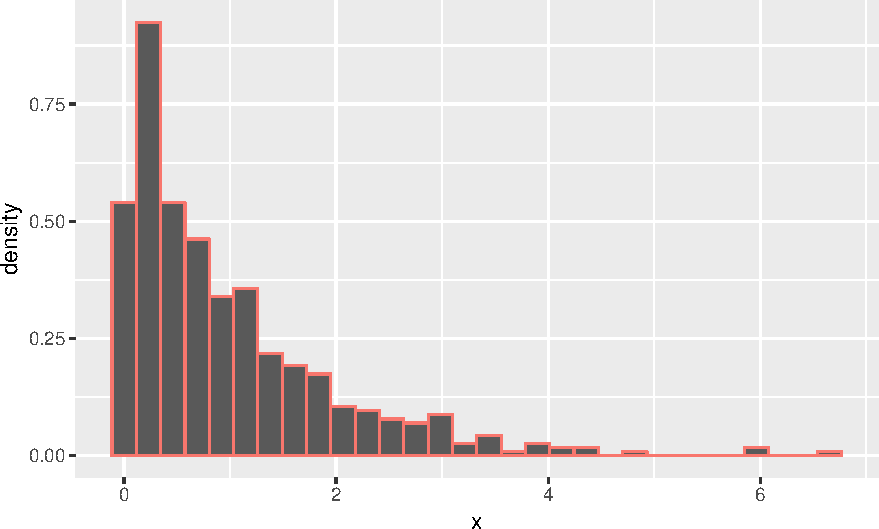
\includegraphics[width=0.7\linewidth]{statistical-computing_files/figure-latex/unnamed-chunk-10-1} \end{center}

\subsection{Discrete case}\label{discrete-case}

\chapter{Monte Carlo Integration and Variance Reduction}\label{mcint}

\bibliography{book.bib,packages.bib}


\end{document}
